%!TEX root = thesis.tex
\chapter{Analysis of the Monitorability of Timing Constraints}

\section{Monitorability of the TADL2 Timing Constraints}
	In this chapter, each of the TADL2 constraints will classified into the classes \emph{Simple Monitorable}, \emph{Simple Monitorable with Delay} and \emph{Not Simple Monitorable}, like defined in chapter~\ref{chapter-monitorability}. For the last class, it will be demonstrated, if the constraint is not simple monitorable in any cases or just in worst case scenarios.

\subsection{DelayConstraint}
	\label{monitorability_DelayConstraint}
	The \emph{DelayConstraint} is defined as\\[10pt]
	\begin{math}
		\forall x\in source:\exists y\in target: lower\leq y-x\leq upper.
	\end{math}\\[10pt]
	and describes that in the time interval between $lower$ and $upper$ after any $source$ event, there is at least one $target$ event. Therefore, the state that need to be stored to monitor the \emph{DelayConstraint} is the set of $source$ events, that are younger than $upper$ and did not have a matching $target$ event yet. If this information is not stored, the constraint cannot be monitored correctly. Updates to this state and output of the monitor are done at $source$ and $target$ events and at delay timestamps $upper$ after the oldest stored $source$ event.\\
	The maximal required storage size of the state depends on the number of $source$ events, which can possibly occur in any time interval of the length $upper$. An example of this worst case situation can be seen in figure~\ref{fig:DelayConstraintWorstCase}. The attributes in this example are $lower=upper=5$, $source$ events occur in the timestamps $\{1, 1.1, ..., 5.9\}$ and $target$ events in the timestamps $\{6, 6.1, ..., 11\}$. At timestamp 6, all 49 $source$ events must be stored, because they are all required to generate the correct output in this and in following timestamps. At this timestamp, the oldest $source$ event can be removed from the storage, because the matching $target$ event occurs in this timestamp. Other timestamps cannot be removed from the storage, because they are younger than $lower$. With every following $target$ event, the oldest event can be removed from the storage, until every $source$ had its matching $target$ event at timestamp 11.\\
	Because the time domain is understood as real numbers in TADL2, a possibly infinite number of events can be placed in any interval of the length $upper$. Which means that the required storage space can grow infinitely, therefore, the worst case memory requirement is dependent of the events in the trace. Consecutively, the \textit{DelayConstraint} is not \textit{simple monitorable}.\\
	Because the $source$ events are removed from the state, when a matching $target$ event occurs, the required storage space does not grow continuously and infinite resources are only required in worst case scenarios. Therefore, the \emph{DelayConstraint} is \emph{worst case not simple monitorable}.
	\begin{figure}
		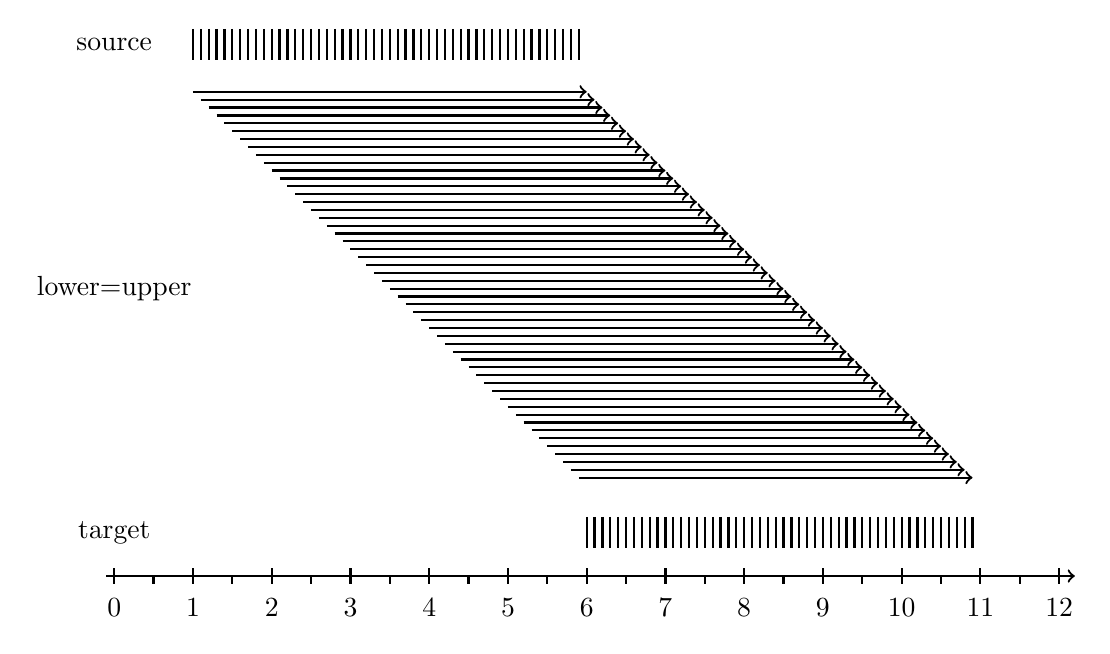
\begin{tikzpicture}[thick]
			\node at (0, 0){source};
			\node at (0, -3.1) {lower=upper};
			\node at (0, -6.2) {target};
			
			%lower = 5, upper = 5
			\foreach \x in {1.0,1.1, ...,  6}{
				% source
				\draw (\x, 0.2) -- (\x, -0.2);
				% target
				\draw (\x+5, -6) -- (\x+5, -6.4);
			}
			
			% lower/upper
			\foreach \x in {0, 0.1, ..., 5}{
				\draw[->] (1 + \x, -0.6-\x) -- (6+\x, -0.6-\x);
			}
			
			\foreach \y in {-6.75}{
				\foreach \x in {0, 1, ..., 12}{
					\draw (\x, \y+0.1) -- (\x,  \y-0.1);
					\node at(\x,  \y-0.4) {\x};
				}
				\foreach \x in {0.5, 1.5, ..., 11.5}
				\draw (\x, \y) -- (\x, \y-0.1);
				\draw[->] (-0.1, \y) -- (12.2, \y);
			}
		\end{tikzpicture}
		\caption{\emph{DelayConstraint} or \emph{StrongDelayConstraint}  with $lower=upper=5$}
		\label{fig:DelayConstraintWorstCase}
	\end{figure}
	

	
\subsection{StrongDelayConstraint}
	The difference between the \emph{DelayConstraint} and the \emph{StrongDelayConstraint} is that for every $source$ event, there must be exactly one matching $target$ event in the \emph{StrongDelayConstraint}. Therefore, the state of the monitor is nearly the same. Like before, all $source$ events, that did not have a matching $target$ event yet, must be stored, but at matching $target$ events, only one $source$ event can be removed from the storage. The worst case memory requirement remains unchanged and is still dependent of the number and the placement of the input events, therefore the \emph{StrongDelayConstraint} is \textit{worst case not simple monitorable} with the same argumentation as for the \textit{DelayConstraint}.

\subsection{RepeatConstraint}
	The \emph{RepeatConstraint} defines the time distance between each event and its $span^{th}$ successor. Therefore, the state, that must be stored for monitoring, consists of the timestamps of the $span+1$ latest events. The state is updated at every event, the oldest stored event is removed and the timestamp of the current event is placed in the storage. The output function checks, if the time distance between the oldest stored event and the current timestamp is between $lower$ and $upper$. To monitor this constraint, a single delay is required, because a missing event, or an event that occurs too late, would not be determined in the right timestamp otherwise. The delay offset can be calculated by the time distance between the current timestamp and the timestamp, that lays $upper$ behind the oldest stores event.\\
	Because the memory requirements are fix ($span+1$ timestamps must be stored) and the state transition and output function can be programmed in a way that they are in  $\mathcal O(1)$ (e.g. if double linked lists are used), the \emph{RepeatConstraint} is \textit{simple monitorable with delay}.

\subsection{RepetitionConstraint}
	The \emph{RepetitionConstraint} is defined as\\[10pt]
		$RepetitionConstraint(s, lower, upper, span, jitter)$\\
		$\equiv \exists X\subset \mathbb{T}: RepeatConstraint (X, lower, upper, span)$\\
		\hspace{7cm}$\land$ $StrongDelayConstraint(X, s, 0, jitter)$\\[10pt]
	The elements of the set $X$ follow the RepeatConstraint and the events, which should be monitored, are following in an interval of the length $jitter$ after the elements of $X$. For each element of $X$, there is exactly one event in $s$ and vice versa.\\
	The monitoring algorithm for this constraint, which will be explained in detail in \ref{chapter-implementation}, stores the upper and lower bounds for the next $span$ elements of $X$.
	These borders are stored in a list and calculated by\\[10pt]
	$lowerBound:= List\_append(last(List\_tail(LowerBound), s), lowerBoundNow + lower)$ \\for the lower bound and\\
	$upperBound:= List\_append(last(List\_tail(UpperBound), s), upperBoundNow + upper)$ \\for the upper bound.\\[10pt]
	The oldest item in these lists (the head of these lists) are removed and the newly calculated bounds for the $span$ next element of $X$ is inserted at the lists end. $lowerBoundNow$ and $upperBoundNow$ are the describing the limitations of the element of $X$ right before the current event. They are calculated using the list mentioned above and the timestamp of the current event by the following definition:\\[10pt]
	$lowerBoundNow:= max(List\_head(last(LowerBoundX, s)), time(s)-jitter)$\\
	$upperBoundNow:= min(List\_head(last(UpperBoundX, s)), time(s))$\\[10pt]
	If the timestamp of the current event is between $lowerBoundNow$ and $upperBoundNow$, the output of the monitor is $true$, in any other case, or when the delay ran out, it is $false$.\\
	The size of these lists has a fixed upper limit ($span$) and the state transition and output functions are in $\mathcal{O}(1)$, therefore they are independent from the trace and the \emph{RepetitionConstraint} is a property, which is \textit{simple monitorable with delay}.
	
\subsection{SynchronizationConstraint}
	The \emph{SynchronizationConstraint} describe groups of streams, which events occur in common clusters. Each of these streams must have at least one event in each of these intervals. Any events, that lay outside of these intervals are prohibited.\\
	Figure~\ref{fig:SynchronizationConstraintWorstCase}, which is similar to the example for the \emph{DelayConstraint}, shows an example of this constraint, which is an worst case scenario in terms of monitoring. The $tolerance$ interval is 5 timestamps long, the event set $s_1$ contains the events $\{1, 1.1, ..., 5.9\}$ and $s_2$ is containing $\{6, 6.1, ..., 11\}$. Each of the events of $s_1$ must be stored until the end of the $tolerance$ interval, otherwise it would be impossible to check the constraint correctly. Like described in section~\ref{monitorability_DelayConstraint}, an arbitrary number of events can be placed in this interval and the memory requirements are dependent of the input streams. The required storage space is not growing continuously, because the stored events can be removed at the end of the $tolerance$ interval, therefore the \emph{SynchronizationConstraint} is \textit{worst case not simple monitorable}.\\
	\\
	It should be noted, that the illustration of the constraint in figure~\ref{fig:SynchronizationConstraintWorstCase} may be misleading, because the $tolerance$ intervals are only shown after the events of $s_1$, not after the events of $s_2$. Every implementation of a monitor for this constraint must also store the events of $s_2$ for the length of $tolerance$, as they could be important for events following after them.
	\begin{figure}
		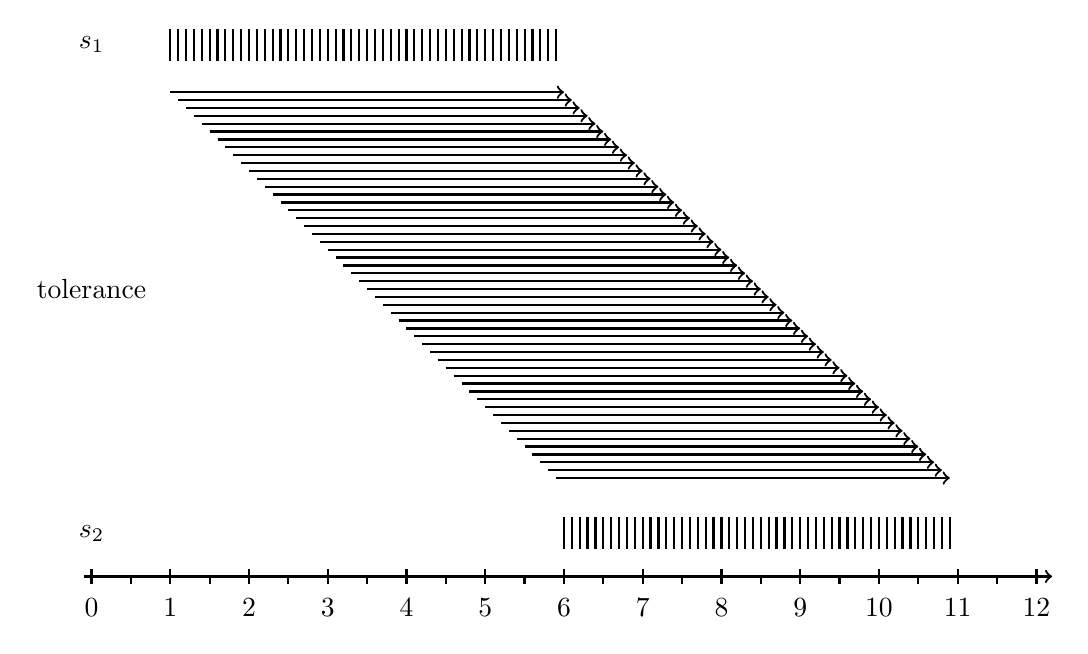
\begin{tikzpicture}[thick]
			\node at (0, 0){$s_1$};
			\node at (0, -3.1) {tolerance};
			\node at (0, -6.2) {$s_2$};
			
			%lower = 5, upper = 5
			\foreach \x in {1.0, 1.1, ...,  6}{
				% source
				\draw (\x, 0.2) -- (\x, -0.2);
				% target
				\draw (\x+5, -6) -- (\x+5, -6.4);
			}
			
			% lower/upper
			\foreach \x in {0, 0.1, ..., 5}{
				\draw[->] (1 + \x, -0.6-\x) -- (6+\x, -0.6-\x);
			}
			
			\foreach \y in {-6.75}{
				\foreach \x in {0, 1, ..., 12}{
					\draw (\x, \y+0.1) -- (\x,  \y-0.1);
					\node at(\x,  \y-0.4) {\x};
				}
				\foreach \x in {0.5, 1.5, ..., 11.5}
				\draw (\x, \y) -- (\x, \y-0.1);
				\draw[->] (-0.1, \y) -- (12.2, \y);
			}
		\end{tikzpicture}
		\caption{\emph{SynchronizationConstraint} or \emph{StrongSynchronizationConstraint}  with $tolerance=5$}
		\label{fig:SynchronizationConstraintWorstCase}
	\end{figure}
	
	
\subsection{StrongSynchronizationConstraint}
	The difference between the \emph{StrongSynchronizationConstraint} and the \emph{SynchronizationConstraint} is, that in the StrongSynchronizationConstraint, only one event per stream is allowed per synchronization cluster. Overlapping of these clusters is still possible. Therefore, this constraint can be classified as \textit{worst case not simple monitorable} with the same argumentation as the previous constraint.
	
	
\subsection{ExecutionTimeConstraint}
	The \emph{ExecutionTimeConstraint} ensures that the time distance between $stop$ and $start$ events, not counting interruptions (which are specified by $preempt$ and $resume$ events) is between $lower$ and $upper$.\\
	Under the assumption that the input events are in logical order (every execution is started by an $start$ event and finished by an $stop$ event, every $preempt$ event is followed by an $resume$ event with no other event in between and no $preempt$ or $resume$ events occur outside of the intervals spanned by $start$ and $stop$ events), three time values must be stored to monitor this constraint. First, the timestamp of the latest $start$ event. Second, the timestamp of the latest $preempt$ event and third, the sum of the time distances between the $resume$ and $preempt$ events. This sum is resetted at every $start$ event.\\
	These values are updated on events in $start$, $preempt$ and $resume$.\\
	For the output function, the run time can be calculated by\\ $runtime = time(now) - time(start) - (sum(time(resume) - time(preempt))$.\\ At any event, this value must smaller or equal to $upper$ and at events in $stop$, additionally the runtime must be greater or equal to $lower$. \\
	To monitor this constraint correctly, a delay is required, when a $stop$ event is late or missing. The delay duration is the distance between the current timestamp and $upper$ minus $runtime$ after the current timestamp.\\
	The required storage space is fixed(remind, that we limited the memory size of timestamps in \ref{monitorability_timestamps}), also the runtime of the state transition and output function can be implemented with constant run time, consecutively the \emph{ExecutionTimeConstraint} is \textit{simple monitorable with delay}.


\subsection{OrderConstraint}
	The \emph{OrderConstraint} describes that an $i^{th}$ $target$ event must exist, if an $i^{th}$ $source$ event exists and that the $i^{th}$ $target$ event occurs after the $i^{th}$ $source$ event. In a finite setting, it must also be checked that the number of $source$ and $target$ events is equal in the end of the observation. Because it is possible that an arbitrary large number of $source$ events occur before the first $target$ occurs, a possibly arbitrary large number must be stored, and the required storage space is dependent on the input streams.  Because this is only a worst case scenario and the size of the stored number can be decreased, when a $target$ event occurs, the \emph{OrderConstraint} is \textit{worst case not simple monitorable}.
	
\subsection{ComparisonConstraint}
	The \textit{ComparisonConstraint} defines an ordering relation between two single events and does not describe relations of streams or their events. Therefore, the definition of \textit{simple monitorability} is not applicable. But because of the restrictions to timestamps made in section~\ref{monitorability_timestamps}, the maximal required storage space and the run time of the operators $\leq, <, \geq, >, =$ have a fixed upper limit.
	
\subsection{SporadicConstraint}
	The \emph{SporadicConstraint} is defined via the \emph{Repetition-} and \emph{RepeatConstraint} without introducing any new timestamps in the definition of the \emph{SporadicConstraint}. These Constraints are \textit{simple monitorable with delay}, therefore the \emph{SporadicConstraint} is also \textit{simple monitorable with delay}.
	
\subsection{PeriodicConstraint}
	The \emph{PeriodicConstraint} is special application of the \emph{SporadicConstraint}, therefore it is also \textit{simple monitorable with delay}.
	
\subsection{PatternConstraint}
	The \emph{PatternConstraint} was redefined to\\[10pt]
	\begin{math}
		\exists X: PeriodicConstraint(X, period, 0, 0)\\
		\text{\hspace{.5cm}} \land \forall i: StrongDelayContraint(X, event, offset_i, offset_i+jitter)\\
		\text{\hspace{.5cm}} \land RepeatConstraint(event, minimum, \infty, 1)
	\end{math}\\[10pt]
	in section~\ref{sec:patterConstraintDefinition}. The input events occur after the strictly periodic timestamps of $X$. The distances between the elements of $X$ and the following events is defined by \textit{offset}.\\
	This constraint can be monitored by storing the upper and lower limit of the current latest element of $X$ and the number of event occurrences, reset to 0 at every |\emph{offset}|$^{th}$ event. The limits of the elements of $X$ can be narrowed down at every event occurrence, because the valid distance between the event and the element of $X$ is known by \emph{offset} and $jitter$. At every $|\text{\emph{offset}}|^{th}$ event occurrence, the limitations of the current $X$ must be increased by $period$. The validity of the constraint can be tested by checking, that the current event has the correct distance to the limitations of the current latest element of $X$. To be able to recognize late or missing events, a delay is required.The timestamp, where the delay must occur, can be calculated by adding $jitter$ and the entry of \textit{offset} for the next expected event to the current upper limit of latest $X$.\\
	Because the memory requirements (two timestamps and an integer) are constant and the mentioned state transition, delay calculation and evaluation functions can be implemented in constant time, the \emph{PatternConstraint} is \textit{simple monitorable with delay}.\\[10 pt]
	If the redefinition of the \emph{PatternConstraint} is not done, the constraint can be reduced to\\[10pt]
	\begin{math}
		RepeatConstraint(event, minimum, \infty, 1)
	\end{math}\\[10pt]
	like stated before in section~\ref{sec:patterConstraintDefinition}. Because the \textit{RepeatConstraint} is \textit{simple monitorable with delay} and the $upper$ parameter is $\infty$, the constraint is \textit{simple monitorable} (without delay) in this variant.
	
\subsection{ArbitraryConstraint}
	The \emph{ArbitraryConstraint} is defined as combination of the \emph{RepeatConstraint}:\\[10pt]
	\begin{math}
		ArbitraryConstraint(event, minimum_1, ..., minimum_n, maximum_1, ..., maximum_n)\\
		\Leftrightarrow \forall i\in{1, ..., n}: RepeatConstraint(event, minimum_i, maximum_i, i).
	\end{math}\\[10pt]
	The \emph{RepeatConstraint} is \textit{simple monitorable with delay}, therefore the \emph{ArbitraryConstraint} is also \textit{simple monitorable with delay}.
	
\subsection{BurstConstraint}
	The \emph{BurstConstraint} is defined as combination of the \emph{RepeatConstraint}:\\[10pt]
	\begin{math}
		RepeatConstraint(event, length, \infty, maxOccurrences)\\
		\text{\hspace{.5cm}}\land RepeatConstraint(event, minimum, \infty, 1)
	\end{math}\\[10pt]
	The \emph{RepeatConstraint} is \textit{simple monitorable with delay}. The $upper$ parameter in both application of the \textit{RepeatConstraint} is $\infty$, therefore the timeout always occurs infinite timestamps after the latest input events, which means, the timeout is dispensable and the \emph{BurstConstraint} can be monitored without any delay or timeout operator. Consecutively, the \emph{BurstConstraint} is a \textit{simple monitorable} property.

\subsection{EventChains}
	The \textit{ReactionConstraint} and the following Constraints are defined on \textit{EventChains}, which are defined as $stimulus$ and $response$ stream. Each event of these streams has a color attribute, which describes the causal connection of individual events.  It is required, that any $stimulus$ event of a specific color must occur before the first $response$ event with the same color. The datatype of this attribute is not specified, except that it may be infinite and an equality test must exist.\\
	Monitoring this property is difficult, because it is required to store every color which has occurred in $response$. The reason for this can be seen in figure~\ref{fig:colorExample}. In the interval between the timestamps 1 and 2, there are 5 events of different colors in $stimulus$. Their counterparts in $response$ occur in the interval between 4 and 5. In timestamp 6, there is an event in $response$ with of the color black. After that, not black is allowed in $stimulus$. To check this properly for all colors, the color of all events, which occurred in $response$ must be stored until the end of the observation.\\
	The memory consumption to monitor this property is growing continuously with any event that introduces a new color in $response$, therefore the correctness of \textit{EventChains} is a \textit{always not simple monitorable} property.
	\begin{figure}
		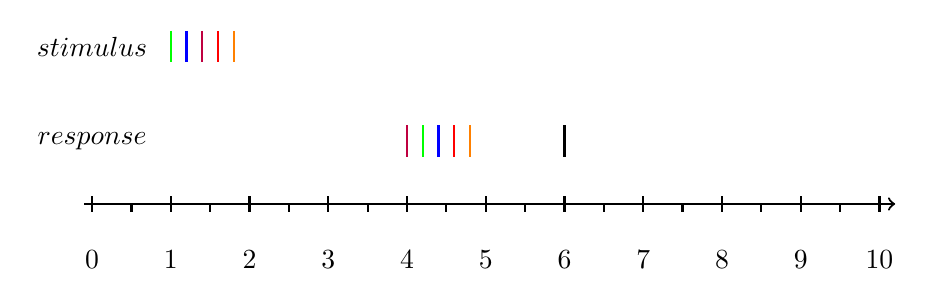
\begin{tikzpicture}[thick]
		\node at (0, 0){$stimulus$};
		\node at (0, -1.2) {$response$};
		%stimulus
		\foreach \x in {0}{
			\draw[green]	(\x + 1  , 0.2) -- (\x + 1  , -0.2);
			\draw[blue]		(\x + 1.2, 0.2) -- (\x + 1.2, -0.2);
			\draw[purple]	(\x + 1.4, 0.2) -- (\x + 1.4, -0.2);
			\draw[red]		(\x + 1.6, 0.2) -- (\x + 1.6, -0.2);
			\draw[orange]	(\x + 1.8, 0.2) -- (\x + 1.8, -0.2);
		}
		%\draw[green]	(8  , 0.2) -- (8 , -0.2);
		%\draw[black]	(9.5  , 0.2) -- (9.5 , -0.2);
		%response
		\foreach \x in {3}{
			\draw[purple]	(\x + 1  , -1) -- (\x + 1  , -1.4);
			\draw[green]		(\x + 1.2, -1) -- (\x + 1.2, -1.4);
			\draw[blue]	(\x + 1.4, -1) -- (\x + 1.4, -1.4);
			\draw[red]		(\x + 1.6, -1) -- (\x + 1.6, -1.4);
			\draw[orange]	(\x + 1.8, -1) -- (\x + 1.8, -1.4);
		}
		\draw[black]	(6, -1) -- (6, -1.4);
		\foreach \y in {-2}{
			\foreach \x in {0, 1, ..., 10}{
				\draw (\x, \y+0.1) -- (\x,  \y-0.1);
				\node at(\x,  \y-0.7) {\x};
			}
			\foreach \x in {0.5, 1.5, ..., 9.5}
			\draw (\x, \y) -- (\x, \y-0.1);
			\draw[->] (-0.1, \y) -- (10.2, \y);
		}
		\end{tikzpicture}
		\centering
		\caption{Event Chain example}
		\label{fig:colorExample}
	\end{figure}
	
\subsection{ReactionConstraint}
	If we assume the correctness of the \textit{EventChains}, a monitor would be similar to a monitor of the \textit{DelayConstraint}. The only difference is that the color attribute of the stored $stimulus$ events must also be stored. Removing events from the storage is only possible, when the time distance and the color between the $stimulus$ and $response$ events is correct.  Like for the \textit{DelayConstraint}, the required worst case storage space is dependent on the input streams, therefore the \textit{ReactionConstraint} is \textit{worst case not simple monitorable}, if the correctness of the \textit{EventChain} is assumed.

\subsection{AgeConstraint}
	Similar to the analysis of the \textit{ReactionConstraint}, we assume the correctness of the \textit{EventChain}.\\
	The \textit{AgeConstraint} is very similar to the \textit{ReactionConstraint}, the main difference is that every $response$ event requires a $stimulus$ event in a matching color in the right distance, not the other way around. Because the $response$ events always occur after the $stimulus$ event(s) in the same color, no delay is required, but the number of events in $stimulus$, that must be stored in worst cases, remains the same as in the \textit{ReactionConstraint}. Therefore, the \textit{AgeConstraint} is \textit{worst case not simple monitorable}, if the correctness of the \textit{EventChain} is assumed.
	
\subsection{OutputSynchronizationConstraint}
	Again, the correctness of the \textit{EventChain} is assumed in the analysis.\\
	The definition of the \textit{OutputSynchronizationConstraint} does not limit the time distance between $stimulus$ events and their associated synchronization clusters in the $response$ streams. If we only consider infinite streams, a missing synchronization cluster cannot make the constraint unsatisfied, therefore, only the correctness of these clusters may be false and lead to a negative output. The correctness of these synchronization clusters is not \textit{simple monitorable}, which is argued the same way as in the simple \textit{SynchronizationConstraint}. An arbitrary large number of new synchronization clusters can be placed in a time interval with the length $tolerance$, which has to be stored until the all $response$ streams have fulfilled this cluster. A key different to the \textit{SynchronizationConstraint} is that only the first occurrences of each color must form a synchronization cluster. After this cluster, events of this color may occur independently. Because of this characteristic, the color of any finished synchronization cluster must be stored for the entire rest of the observation, which means, the \textit{OutputSynchronizationConstraint} is a \textit{always not simple monitorable} property.\\
	If finite streams are considered, the color of all $stimulus$ events must be stored, until the matching synchronization cluster occurs. At the end of the observation, it must be checked, if there was a synchronization cluster for all colors, which occurred in $stimulus$. The classification as \textit{always not simple monitorable} is not affected by this.
	

\subsection{InputSynchronizationConstraint}
	Like before, the correctness of the \textit{EventChains} is assumed.\\
	In the \textit{InputSynchronizationConstraint}, synchronization clusters in the $stimulus$ streams must only be fulfilled, if the associated events are the last of their color in their streams before an associated $response$ event. This means, at least some information for every color, which occurred in the $stimulus$ streams, must be stored, until the $response$ color with the same color.  Because several $response$ events of this color may occur, the information about a fulfilled or unfulfilled synchronization cluster may not be removed from the storage. Otherwise it could not be checked correctly, if there was a synchronization cluster with a matching color. Consecutively, the required storage space grows continuously with every new stimulus color and the constraint is \textit{always not simple monitorable}. 
	
\section{Conclusion}
	

\begin{figure}
	\centering
	\includegraphics[width=\linewidth]{relationBetweenConstraint}
	\caption{Overview over constraints - \textcolor{green}{Simple Monitorable} - \textcolor{red}{Not Simple Monitorable}}
	\label{fig:relationbetweenconstraint}
\end{figure}
Figure~\ref{fig:relationbetweenconstraint} gives an overview, which TADL2 timing constraints are \textit{simple monitorable} and which are not. The \textit{ComparisonConstraint} is not defined on streams, therefore the definition of \textit{simple Monitorability} is not applicable. All simple monitorable constraints, except the \textit{BurstConstraint} require the creation of new timestamps. The other constraints are not simple monitorable, of which the \emph{Input-} and \emph{OutputSynchronizationConstraint} are always not simple monitorable. If the correct order of the \textit{EventChains} is assumed, the \textit{Reaction-} and \textit{AgeConstraint} are only not simple monitorable in worst cases, like the other not simple monitorable constraints.\\
The arrows show, which constraint is defined via other constraints, for example the \emph{RepetitionConstraint} is defined via the \emph{StrongDelay-} and \emph{RepeatConstraint}. It should be noted that constraints, which are defined via not simple monitorable constraints, can be simple monitorable, because of further restrictions, which limit the required storage space or runtime.

	
%\section{ReactionConstraint}
%	The \emph{ReactionConstraint} is defined as:
%	\\[10pt]
%	\begin{math}
%		\forall x\in scope.stimulus: \exists y\in scope.response:\\
%		\text{\hspace{.5cm}}x.color=y.color\\
%		\text{\hspace{.5cm}}\land (\forall y'\in scope.response: y'.color=y.color\Rightarrow y\leq y')\\
%		\text{\hspace{.5cm}}\land minimum \leq y-x \leq maximum
%	\end{math}\\[10pt]
%	%For every event $x$ in $scope.stimulus$, there is an event $y$ in $scope.response$ with the same color. The distance between $x$ and $y$ is specified by $minimum$ and $maximum$.
%	The third line is the most relevant for the classification of monitorability. It says, that additional events in $scope.response$ with the same color of $y$ must occur at or after $y$. Other restrictions to additional events in $scope.response$ are not defined.\\
%	\ref{fig:WorstCaseReactionConstraint} visualizes, where this leads to problems in terms of monitoring. Between the timestamps 1 and 7, there are many events with different colors in $scope.response$ and the constraint is satisfied. In timestamp 8, there is an event in $scope.stimulus$ that has a color that matches with one of the $scope.response$ events, therefore the constraint is not fulfilled anymore.\\
%	The Example shows, that every color of the events that have occurred in $scope.response$ must be stored, to monitor the constraint correctly. Any new $scope.response$ event with a new color will extend the required storage space, but it is not possible to release this storage and still monitor the constraint correctly, therefore the memory requirements grows continuously. The definition of the color attribute of events says, that there is an infinite number of possible colors, therefore infinite memory resources are required for this constraint.
%	These characteristics show that this constraint is always non-finite monitorable.
%	\begin{figure}
%		\begin{tikzpicture}[thick]
%			\node at (0, 0){$stimulus$};
%			\node at (0, -1.2) {$response$};
%			%stimulus
%			\draw[green] (8, 0.2) -- (8, -0.2);
%			%response
%			\foreach \x in {0, ..., 5}{
%				\draw[green]	(\x + 1  , -1) -- (\x + 1  , -1.4);
%				\draw[blue]		(\x + 1.2, -1) -- (\x + 1.2, -1.4);
%				\draw[purple]	(\x + 1.4, -1) -- (\x + 1.4, -1.4);
%				\draw[red]		(\x + 1.6, -1) -- (\x + 1.6, -1.4);
%				\draw[orange]	(\x + 1.8, -1) -- (\x + 1.8, -1.4);
%			}
%			\foreach \y in {-2}{
%				\foreach \x in {0, 1, ..., 10}{
%					\draw (\x, \y+0.1) -- (\x,  \y-0.1);
%					\node at(\x,  \y-0.7) {\x};
%				}
%				\foreach \x in {0.5, 1.5, ..., 9.5}
%				\draw (\x, \y) -- (\x, \y-0.1);
%				\draw[->] (-0.1, \y) -- (10.2, \y);
%			}
%		\end{tikzpicture}
%		\caption{ReactionConstraint - Example with additional events and $minimum=maximum=3$}
%		\label{fig:WorstCaseReactionConstraint}
%	\end{figure}
%%TODO response events before stimulus allowed?
%	
%\newpage
%\section{AgeConstraint}
%	The \emph{AgeConstraint} is defined as \\[10pt]
%	\begin{math}
%	\forall y\in scope.response: \exists x\in scope.stimulus:\\
%	\text{\hspace{.5cm}}x.color=y.color\\
%	\text{\hspace{.5cm}}\land (\forall x'\in scope.stimulus: x'.color=x.color\Rightarrow x'\leq x)\\
%	\text{\hspace{.5cm}}\land minimum \leq y-x \leq maximum
%	\end{math}\\[10pt]
%	It is a turned around counterpart to the \emph{ReactionConstraint}, where each event $y$ of $scope.response$ is preceded by an event $x$ in $scope.stimulus$ with matching color. The distance between these events is defined by the attributes $minimum$ and $maximum$. After the latest event $x$, that matches color with $y$ and is in the right distance (hence after $y-minimum$), no more events with this color are allowed. To monitor this property correctly, it is necessary to store, amongst other things, every color of events, that occurred in $scope.response$.  Figure~\ref{fig:WorstCaseAgeConstraint} visualizes this. In the interval from 5 to 6 there are 5 events in $scope.response$, their matching $scope.stimulus$ events are in the interval from 2 to 3. In timestamp 10, there is an event in $scope.stimulus$, which has a color that matches with an color, that has already been used in $scope.response$. The \emph{AgeConstraint} is not satisfied anymore after this, but to find that out, it is required to know every color, which  has already been used in $scope.response$. Like in the \emph{ReactionConstraint}, the memory requirements for this is growing continuously, therefore the \emph{AgeConstraint} is always non-finite monitorable.
%	
%	\begin{figure}
%		\begin{tikzpicture}[thick]
%		\node at (0, 0){$stimulus$};
%		\node at (0, -1.2) {$response$};
%		%stimulus
%		\draw[green]	(2  , 0.2) -- (2  , -0.2);
%		\draw[blue]		(2.2, 0.2) -- (2.2, -0.2);
%		\draw[purple]	(2.4, 0.2) -- (2.4, -0.2);
%		\draw[red]		(2.6, 0.2) -- (2.6, -0.2);
%		\draw[orange]	(2.8, 0.2) -- (2.8, -0.2);
%		
%		\draw[green]	(10, 0.2) -- (10, -0.2);
%		
%		\foreach \x in {0, 0.1, 0.2, 0.3, 0.4}
%			\draw[<-] (2+\x+\x, -0.5-\x) -- (5+\x+\x, -0.5-\x);
%		%response
%		\draw[green]	(5  , -1) -- (5  , -1.4);
%		\draw[blue]		(5.2, -1) -- (5.2, -1.4);
%		\draw[purple]	(5.4, -1) -- (5.4, -1.4);
%		\draw[red]		(5.6, -1) -- (5.6, -1.4);
%		\draw[orange]	(5.8, -1) -- (5.8, -1.4);
%		\foreach \y in {-2}{
%			\foreach \x in {0, 1, ..., 10}{
%				\draw (\x, \y+0.1) -- (\x,  \y-0.1);
%				\node at(\x,  \y-0.7) {\x};
%			}
%			\foreach \x in {0.5, 1.5, ..., 9.5}
%			\draw (\x, \y) -- (\x, \y-0.1);
%			\draw[->] (-0.1, \y) -- (10.2, \y);
%		}
%		\end{tikzpicture}
%		\caption{AgeConstraint - Example with additional events and $minimum=maximum=3$}
%		\label{fig:WorstCaseAgeConstraint}
%	\end{figure}
%	
%
%\section{OutputSynchronizationConstraint}
%	The \emph{OutputSynchronizationConstraint} is defined as\\[10pt]
%	\begin{math}
%		\forall x\in scope_1.stimulus: \exists t: \forall i: \exists y\in scope_i.response:\\
%			\text{\hspace{.5cm}} x.color = y.color\\
%			\text{\hspace{.5cm}}\land (\forall y'\in scope_i.response: y'.color=y.color \Rightarrow y\leq y')\\
%			\text{\hspace{.5cm}}\land 0\leq y-t\leq tolerance,
%	\end{math}\\[10pt]
%	where every $scope_i$ has the same $stimulus$ events.\\
%	Each $scope_1.stimulus$ event $x$ has an event $y$ in every $scope_i.response$ with the same color. This event $y$ is the first occurrence of this color in $scope_i.response$ and the $y$-events of all $scope_i.response$ do not lay more than $tolerance$ time apart.\\
%	A worst case scenario can be constructed, in which any number of events with different colors is placed in $scope_1.stimulus$. To monitor this constraint correctly, the color of all of these events must be stored, until the $response$ event with matching colors occur. Because an infinite number of colors is possible, infinite storage space is needed to monitor this constraint correctly. The colors of the events can be removed from the storage, after the first occurrence of them in the $response$ events, therefore the required memory is not growing continuously and the constraint is worst case Non-Finite monitorable.
%	
%\section{InputSynchronizationConstraint}
%	The \emph{InputSynchronizationConstraint} is defined as\\[10pt]
%	\begin{math}
%		\forall y\in scope_1.response: \exists t: \forall i: \exists x\in scope_i.stimulus:\\
%		\text{\hspace{.5cm}} x.color = y.color\\
%		\text{\hspace{.5cm}}\land (\forall x'\in scope_i.stimulus: x'.color=x.color \Rightarrow x\leq x')\\
%		\text{\hspace{.5cm}}\land 0\leq x-t\leq tolerance
%	\end{math}\\[10pt]
%	and offers an turned around counterpart to the \emph{OutputSynchronizationConstraint}. The synchronized event clusters occur in the $scope_i.stimulus$ events and the latest events of them must be part of the synchronization. Like for the \emph{OutputSynchronizationConstraint} a worst case scenario, where an possibly infinite number of event colors must be stored, can be constructed, by putting a possibly infinite large number of synchronized events into the $scope_i.stimulus$ event sets, before the first event occurs in $scope_1.response$. Similar to the  \emph{OutputSynchronizationConstraint}, the colors of these events must be stored, until they are released by the $response$ events with a matching color, therefore infinite memory resources are required to monitor this constraint correctly and the \emph{InputSynchronizationConstraint} is worst case Non-Finite monitorable.